\documentclass{beamer}
\usepackage{pgfpages}
\usepackage[utf8]{inputenc}
\usepackage{times}
\usepackage{tikz}
\usetheme{Warsaw}
\setbeamercovered{transparent}
%\usecolortheme{seahorse}
\useoutertheme{infolines}
\setbeamertemplate{footline} [frame number]
\title{Automatic identification of landmarks by shape recognition}
%\author{LE Van Linh}
%\institute{LaBRI laboratory}
%\date{\today}
\begin{document}
\frame{\titlepage}
\begin{frame}{Contents}
	\tableofcontents
\end{frame}
\section{Introduction}
%\begin{frame}{Introduction}
%	\begin{itemize}
%		\item Implementation of article \textit{``Automatic identification of landmarks in digital images" $^{\cite{palaniswamy}}$ }
%		\item Examination based on two set of images: \textit{mandibule droite} and \textit{mandibule gauche} 		  
%	\end{itemize}
%\end{frame}
\begin{frame}{Introduction}
	\begin{itemize}
	\item The implementation based on \textbf{"Automatic identification of landmarks in digital images"}, \textit{Palaniswamy, Sasirekha, Neil A. Thacker, and Christian Peter Klingenberg} \\
	\item It includes four steps:
		\begin{center}
			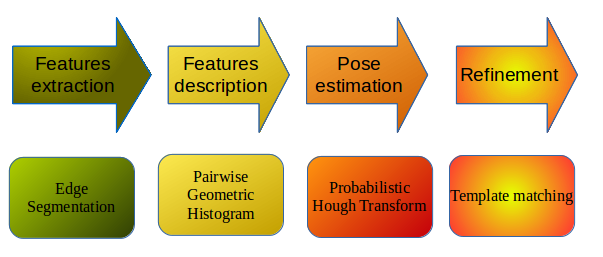
\includegraphics[height=3.5cm]{images/flow_step.png}	
		\end{center}
	\end{itemize}
\end{frame}
\section{Method}
%\subsection{Segmentation}
\begin{frame}{Method - Edge segmentation}
	Purpose: 
	\begin{itemize}
		\item Extract the features (edge) from images
		\item Get the approximate lines
	\end{itemize}
	Method:
	\begin{itemize}
		\item Indicate the threshold value by analysis histogram of image		
		\item Canny
		\item Break edge algorithm
	\end{itemize}
	Parameters:
	\begin{itemize}
		\item Threshold value: indicated by histogram analysis
		\item Canny ratio: 1:3 (lower:upper)
		\item Minimum distance to stop break edge: 3 pixels
	\end{itemize}
\end{frame}
\begin{frame}{Method - Edge segmentation}
	\begin{columns}[c]
		\column{0.5\textwidth}
		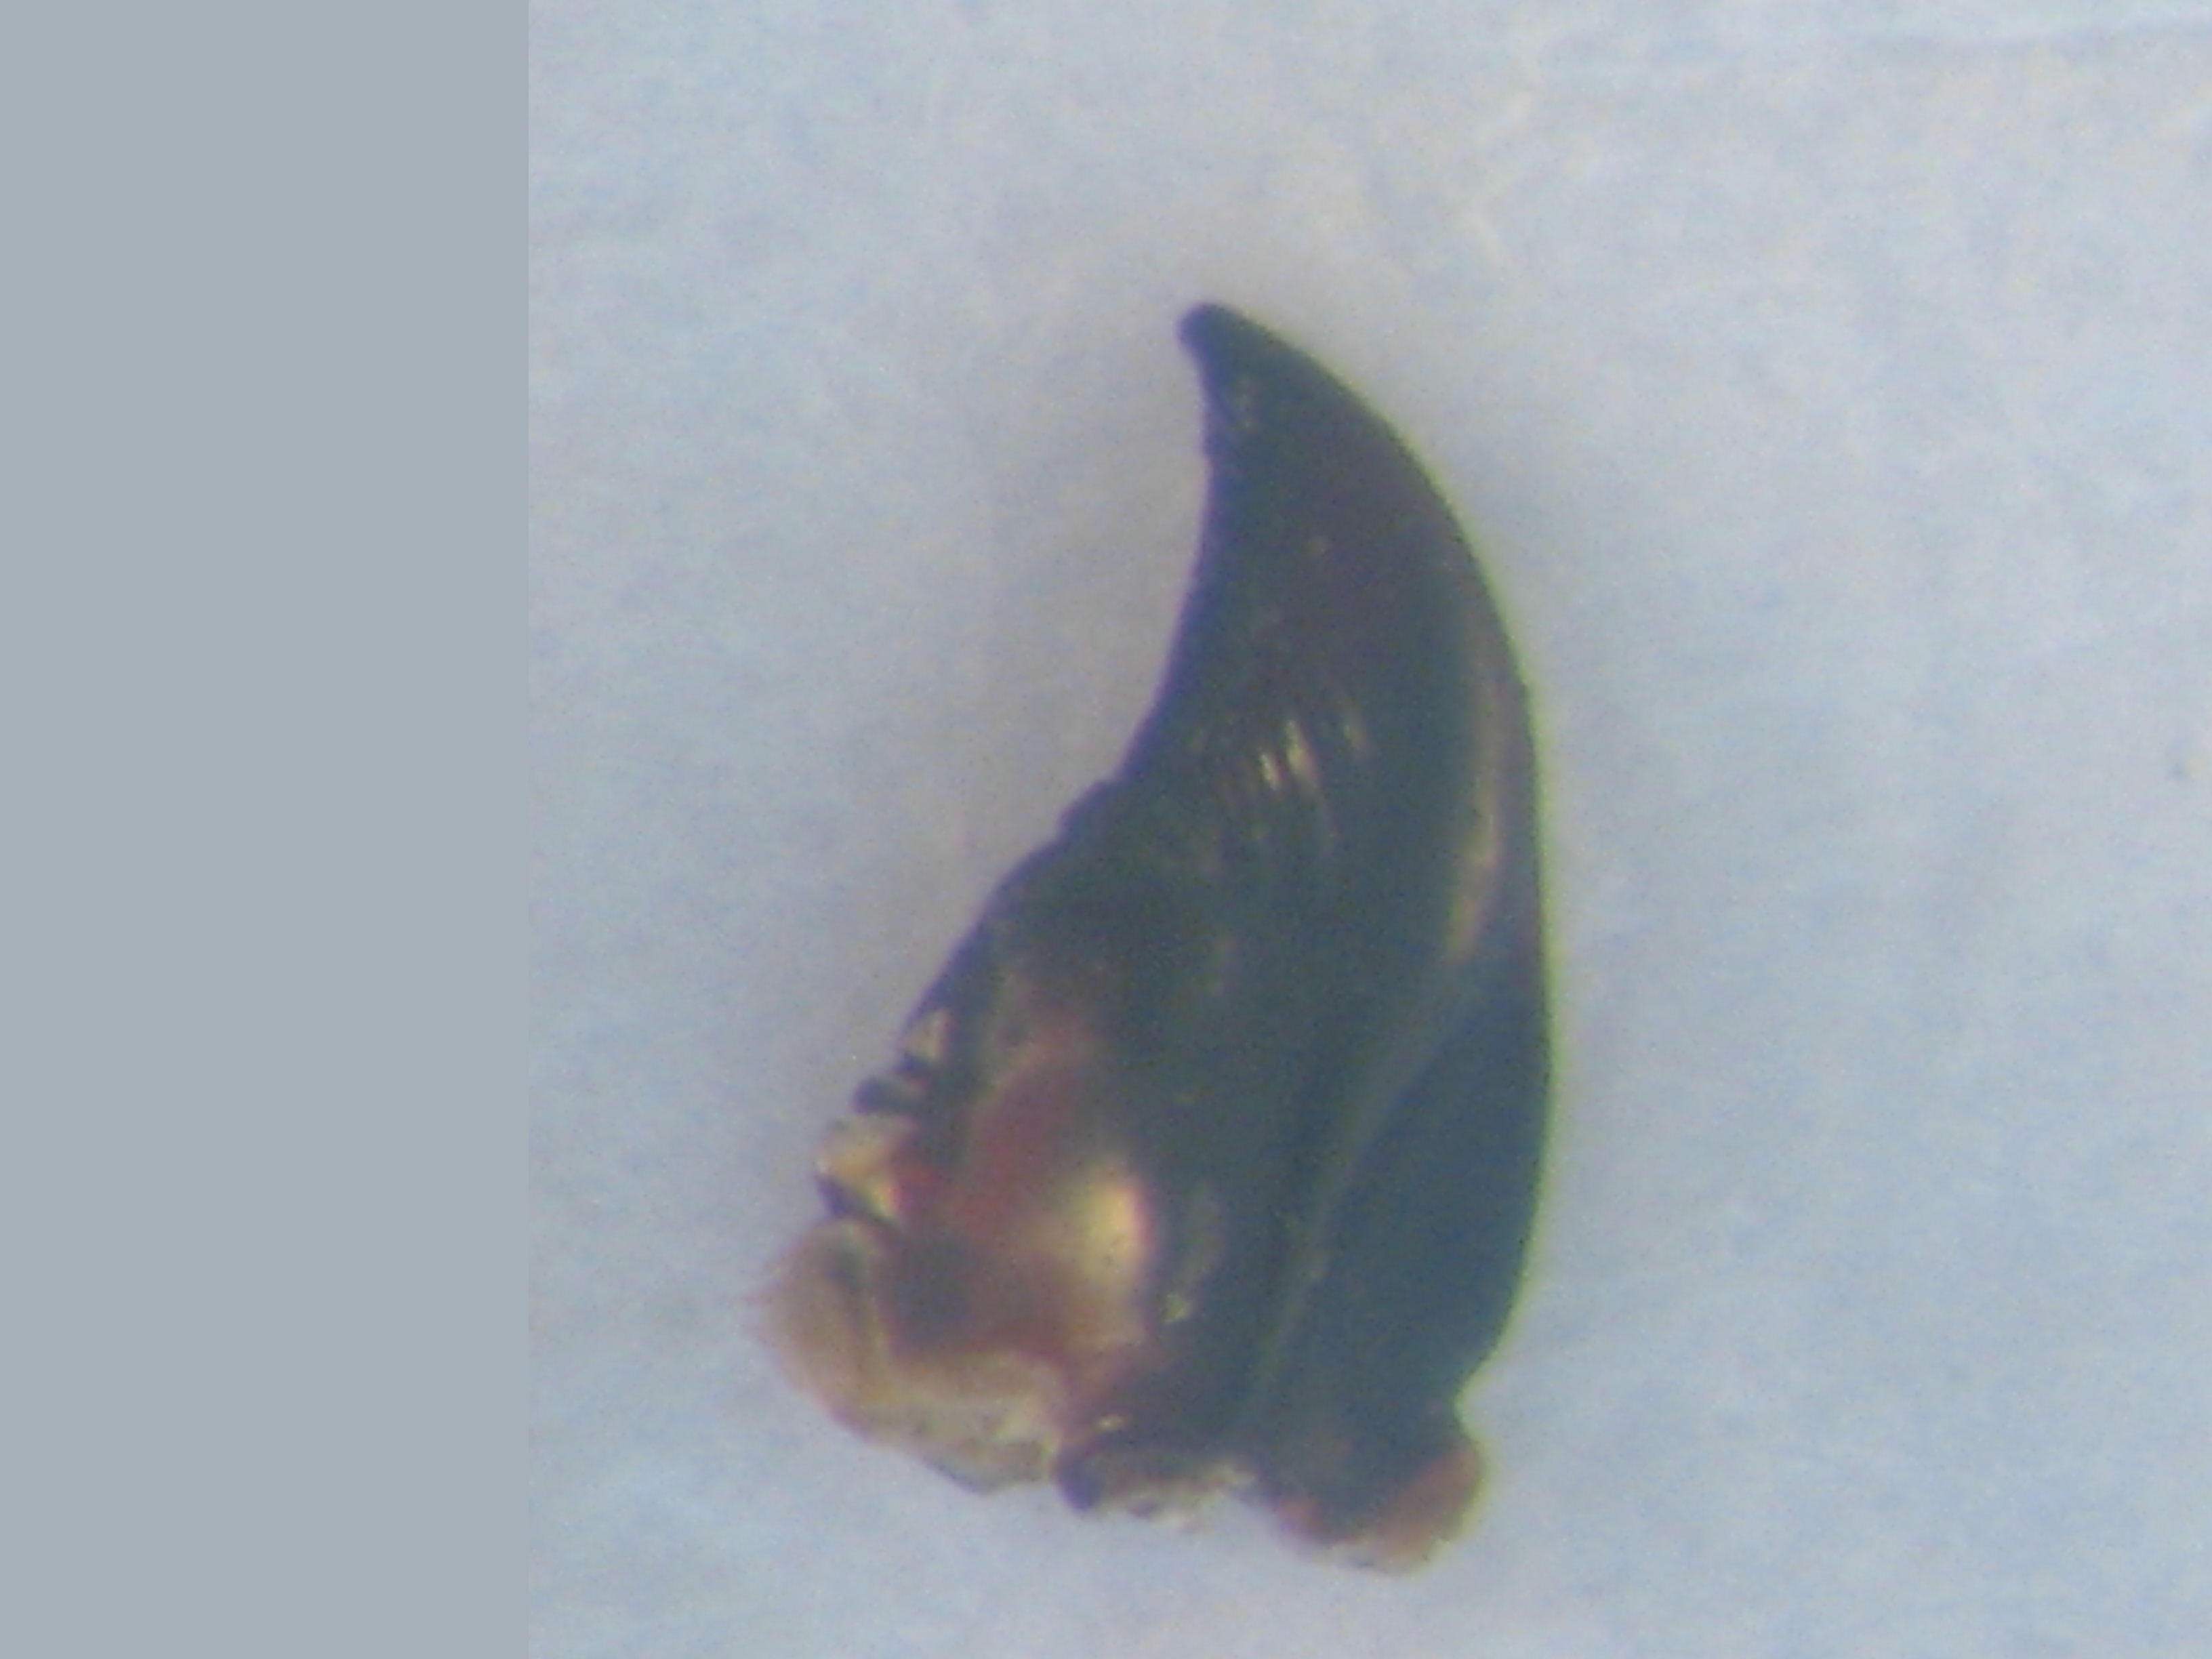
\includegraphics[height=4.5cm]{images/model28.JPG}
		\column{0.5\textwidth}
		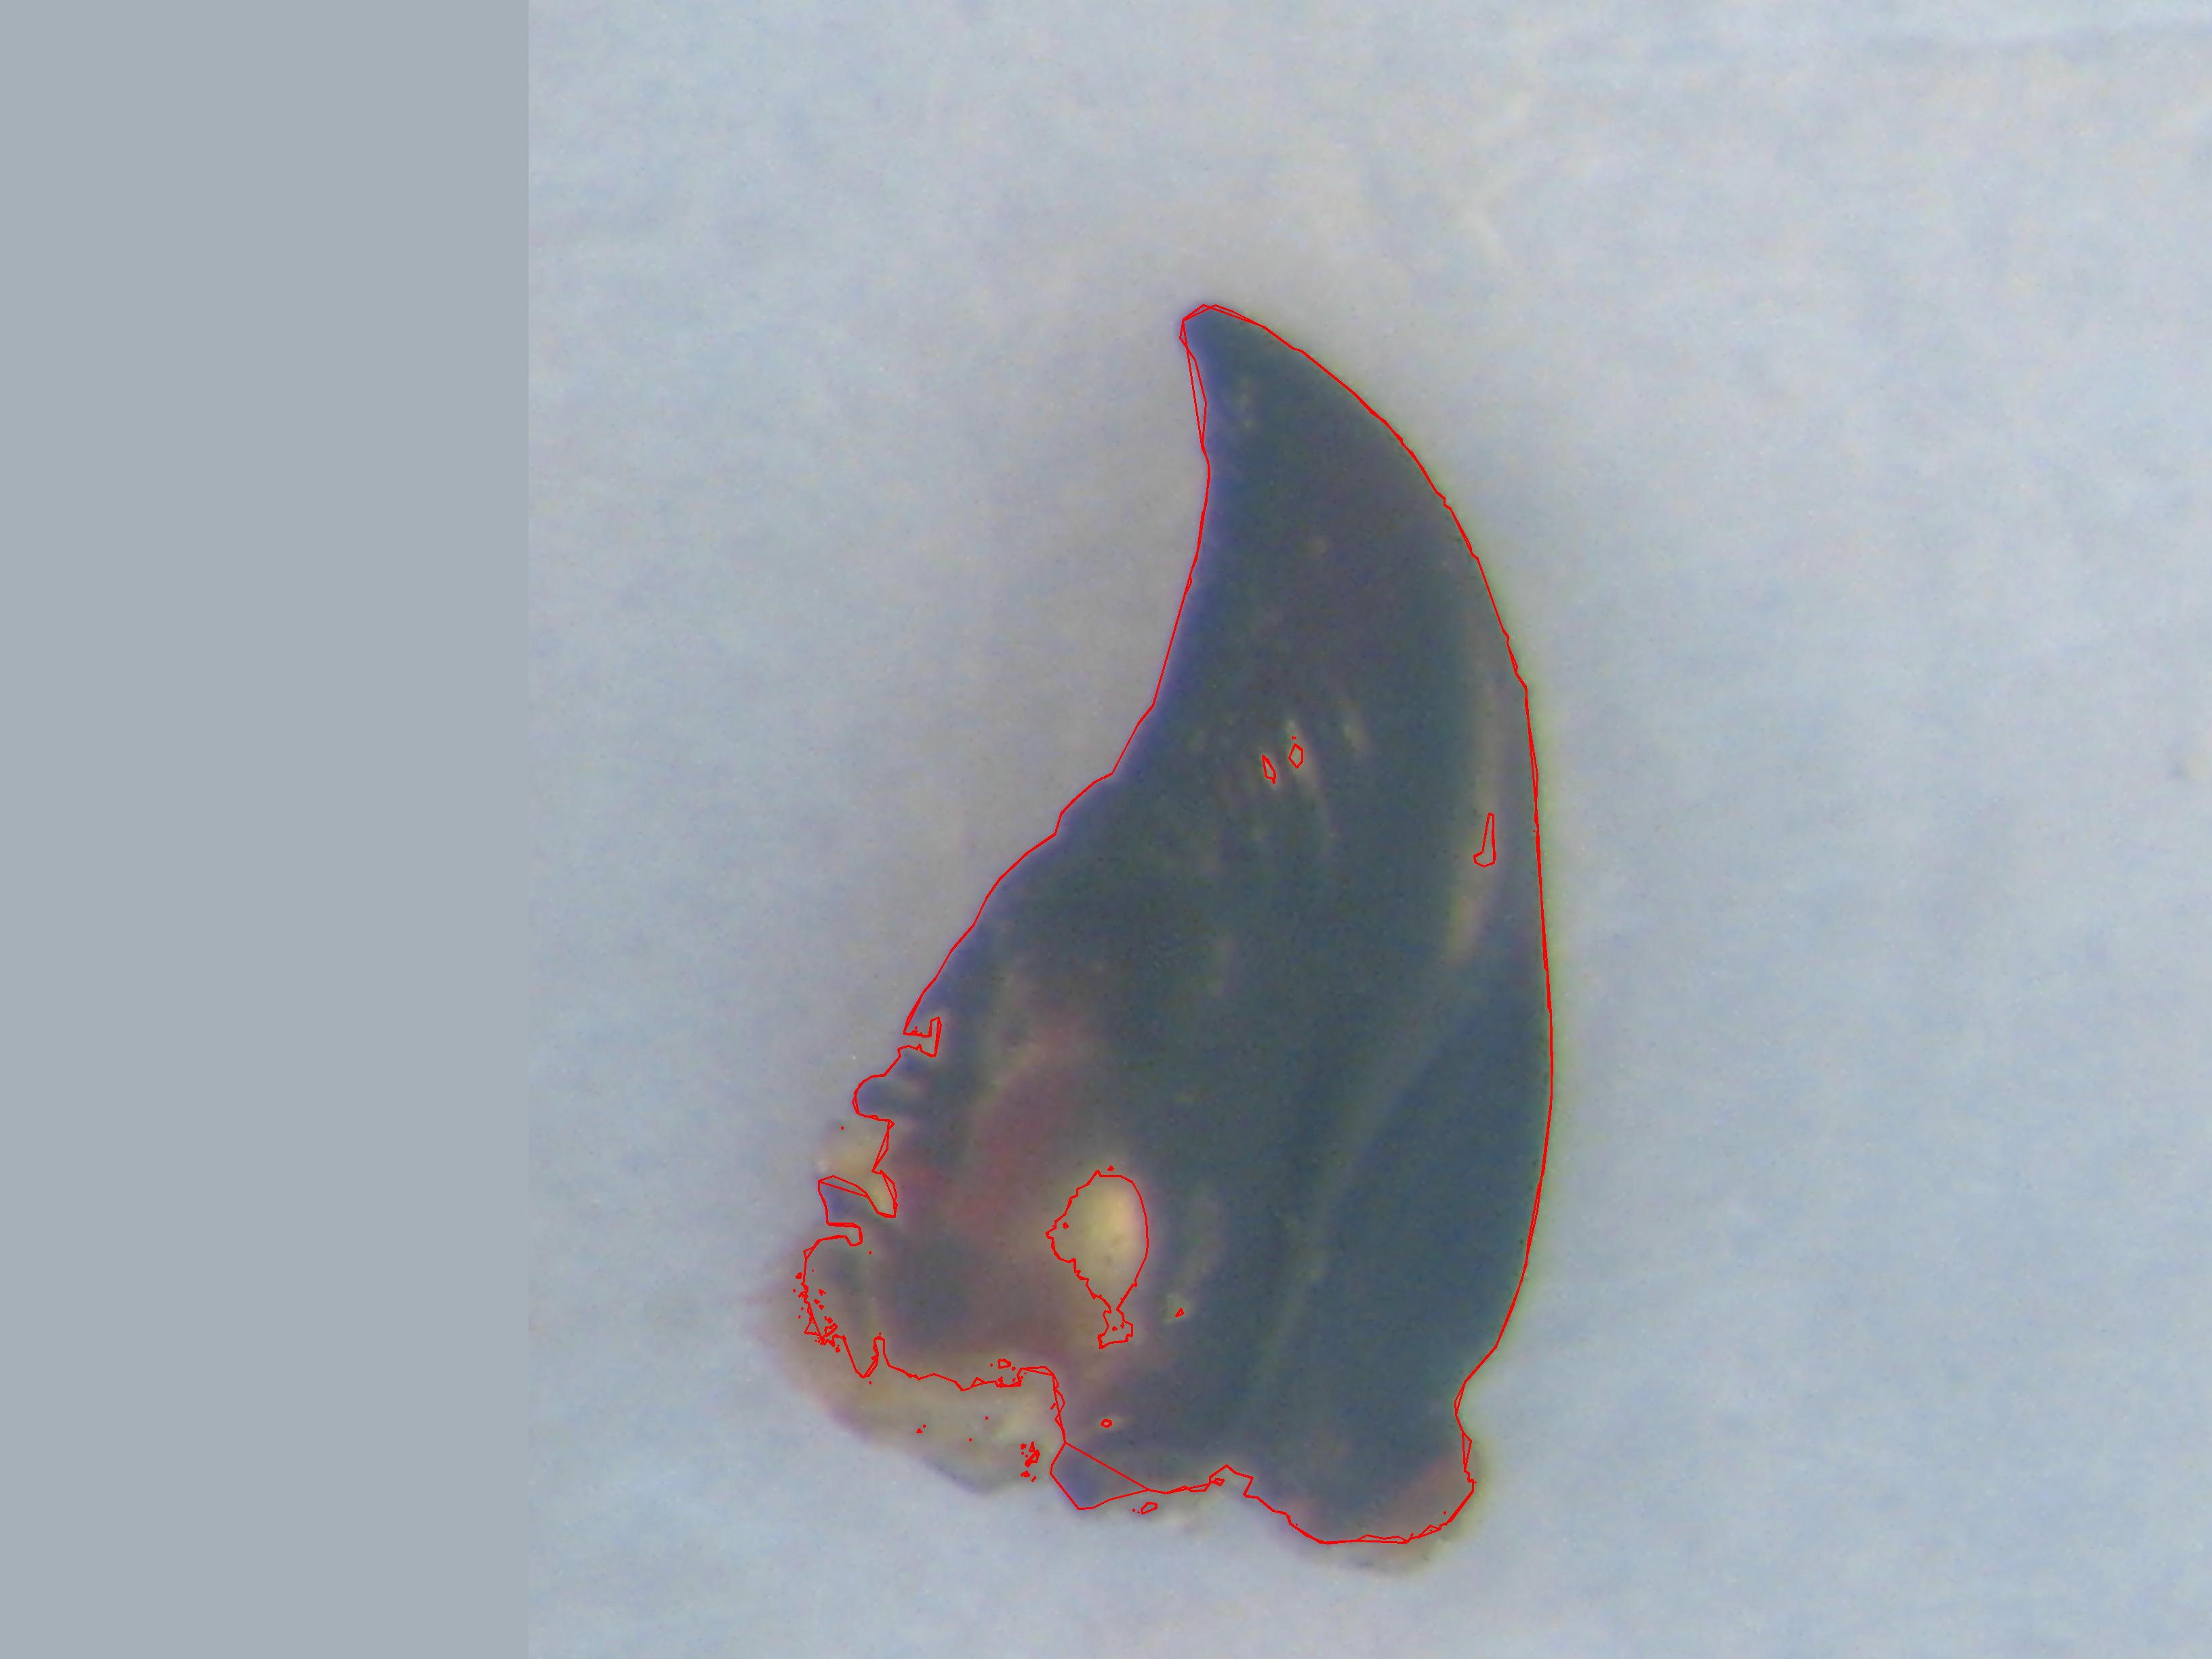
\includegraphics[height=4.5cm]{images/edge28.jpg}
	\end{columns}
\end{frame}
%\subsection{Pairwise geometric histogram(PGH)}
\begin{frame}{Method - Pairwise geometric histogram}
	\begin{description}
		\item[Purpose:] detecting the present of scene image in model image
		\item[Method$^{\cite{pgh}}$:]
		\begin{itemize}
			\item Construct the local PGH
			\item Construct the shape PGH
			\item Matching shape's PGH by Bhattacharyya metric
		\end{itemize}
		\item[Parameters]: to construct the PGH matrix (used to compute the metric)
			\begin{itemize}
				\item Angle accuracy: 90, 180, 360, 720
				\item Distance accuracy: 250, 500, 1000
			\end{itemize}
	\end{description}
\end{frame}
\begin{frame}{Method - Pairwise geometric histogram}
	\framesubtitle{Local PGH and shape PGH}
	\begin{description}
		\item[Local PGH]: PGH for each feature (line)
		\item[Shape PGH]: contains many \textbf{Local PGH}
		\item[PGH]: a matrix two dimensions: angle axis and distance axis
		\item[PGH information]: angle between two lines and perpendicular distance from two endpoints of scene line to reference line.
	\end{description}
\end{frame}
%\subsection{Probabilistic Hough Transform}
\begin{frame}{Method - Probabilistic Hough Transform}
	\begin{description}
		\item[Purpose:]
			\begin{itemize}
				\item Determine the presence and location of model image in scene image
				\item Estimate the landmarks in the scene image
			\end{itemize}
		\item[Method:]
		\begin{itemize}
			\item Construct the reference table
			\item Find the pair scene lines have the best ``vote"
			\item Estimate the ``reference point" in scene image
			\item Estimate the landmarks
		\end{itemize}
		\item[Result:] Estimated model landmarks on scene image
	\end{description}
\end{frame}
\begin{frame}{Method - PHT Parameters}
	\begin{itemize}
		\item Closet lines
			\begin{itemize}
				\item Minimum length of each line: 60 pixels
				\item Minimum angle between two lines: 15 degrees
				\item Distance from an endpoint of a line to another line: 5 pixels
			\end{itemize}
		\item Similar pairs		
			\begin{itemize}
				\item Maximum difference angle: 1 degree
				\item Maximum difference scale: 1 pixel
				\item Maximum difference position: 2 pixels
			\end{itemize}
	\end{itemize}
\end{frame}
\begin{frame}{Method - Probabilistic Hough Transform}
	\begin{center}
		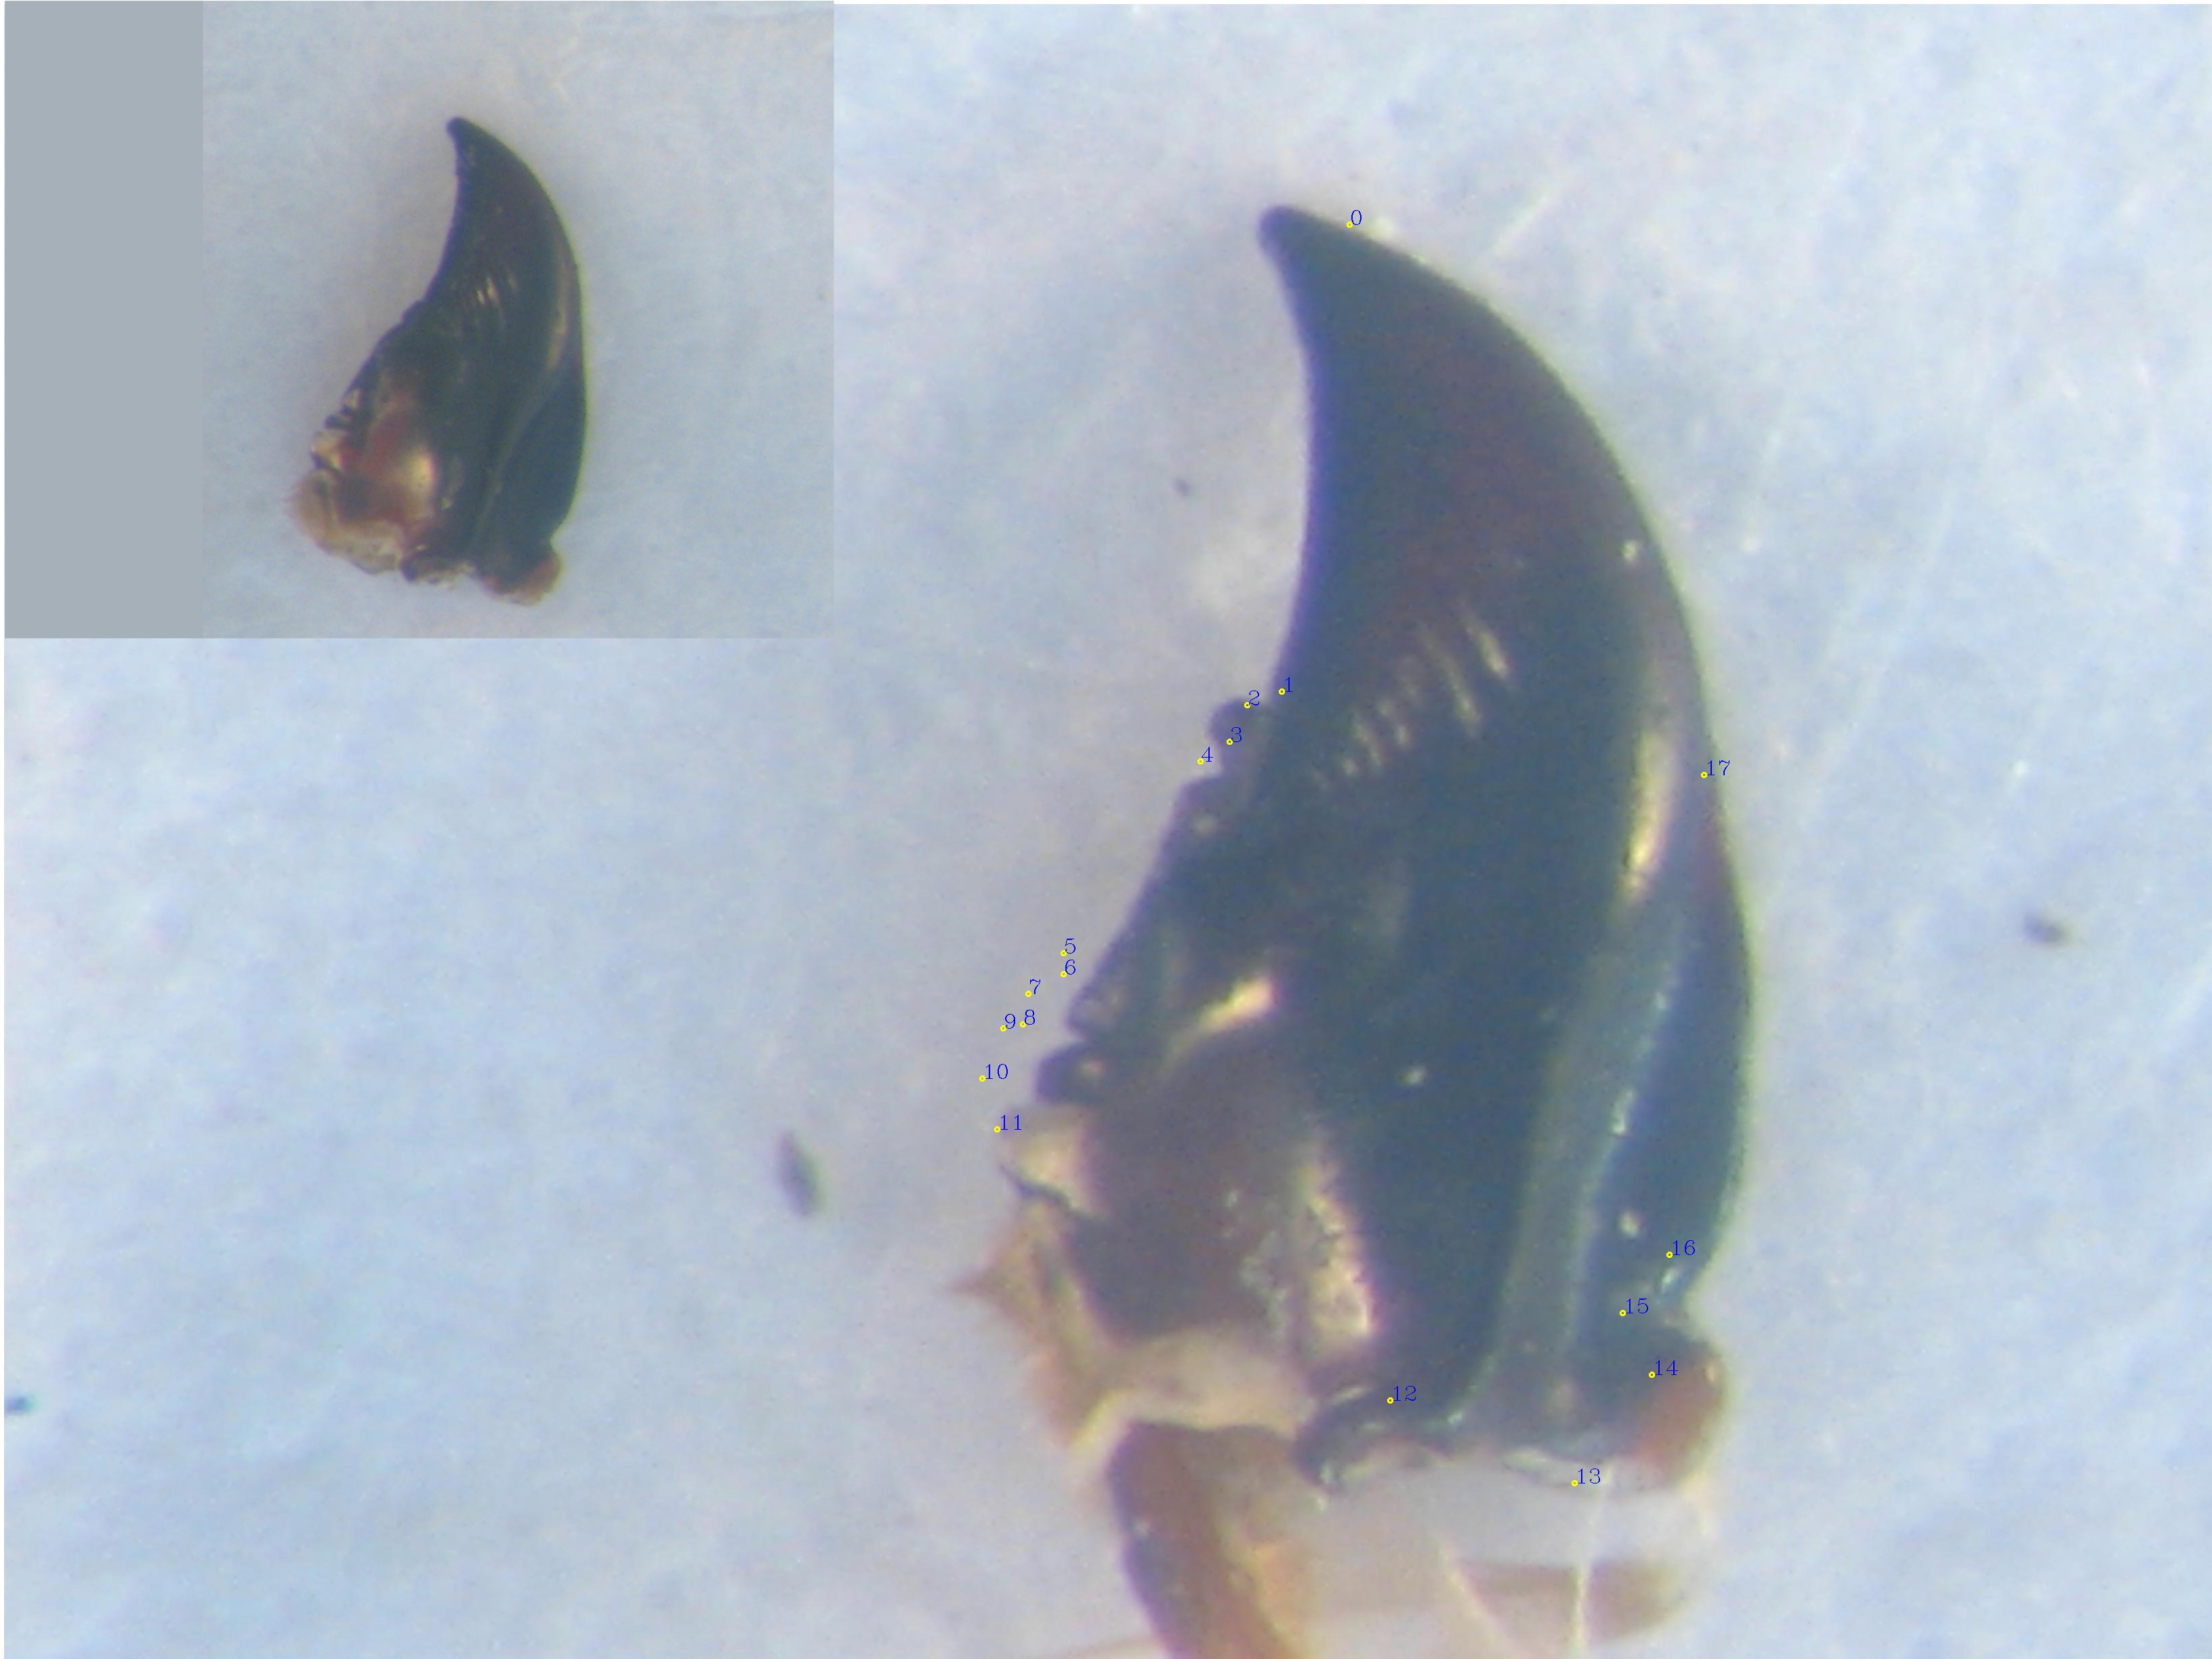
\includegraphics[height=8cm]{images/pht19.JPG}	
	\end{center}
\end{frame}
%\subsection{Template matching}
\begin{frame}{Method - Template matching}
	\begin{description}
		\item [Purpose:] Refine the estimated landmarks on the scene image 
		\item [Method:] 
			\begin{itemize}
				\item On model image: For each landmark, create a bounding box with size ``\textit{t1}" and \textit{landmark} is center point of box
				\item Rotate scene image to match with model
				\item On scene image: For each estimated landmark, create a bounding box with size ``\textit{t2}" and \textit{landmark} is center point of box
				\item Sliding \textit{t1} on \textit{t2} and find the the best match (cross-correlation)
			\end{itemize}
		\item [Parameters:]
			\begin{itemize}
				\item Template box size: 400px
				\item Image box size: 1400px
			\end{itemize}
	\end{description}
\end{frame}
\begin{frame}{Method - Template matching}
	\begin{center}
		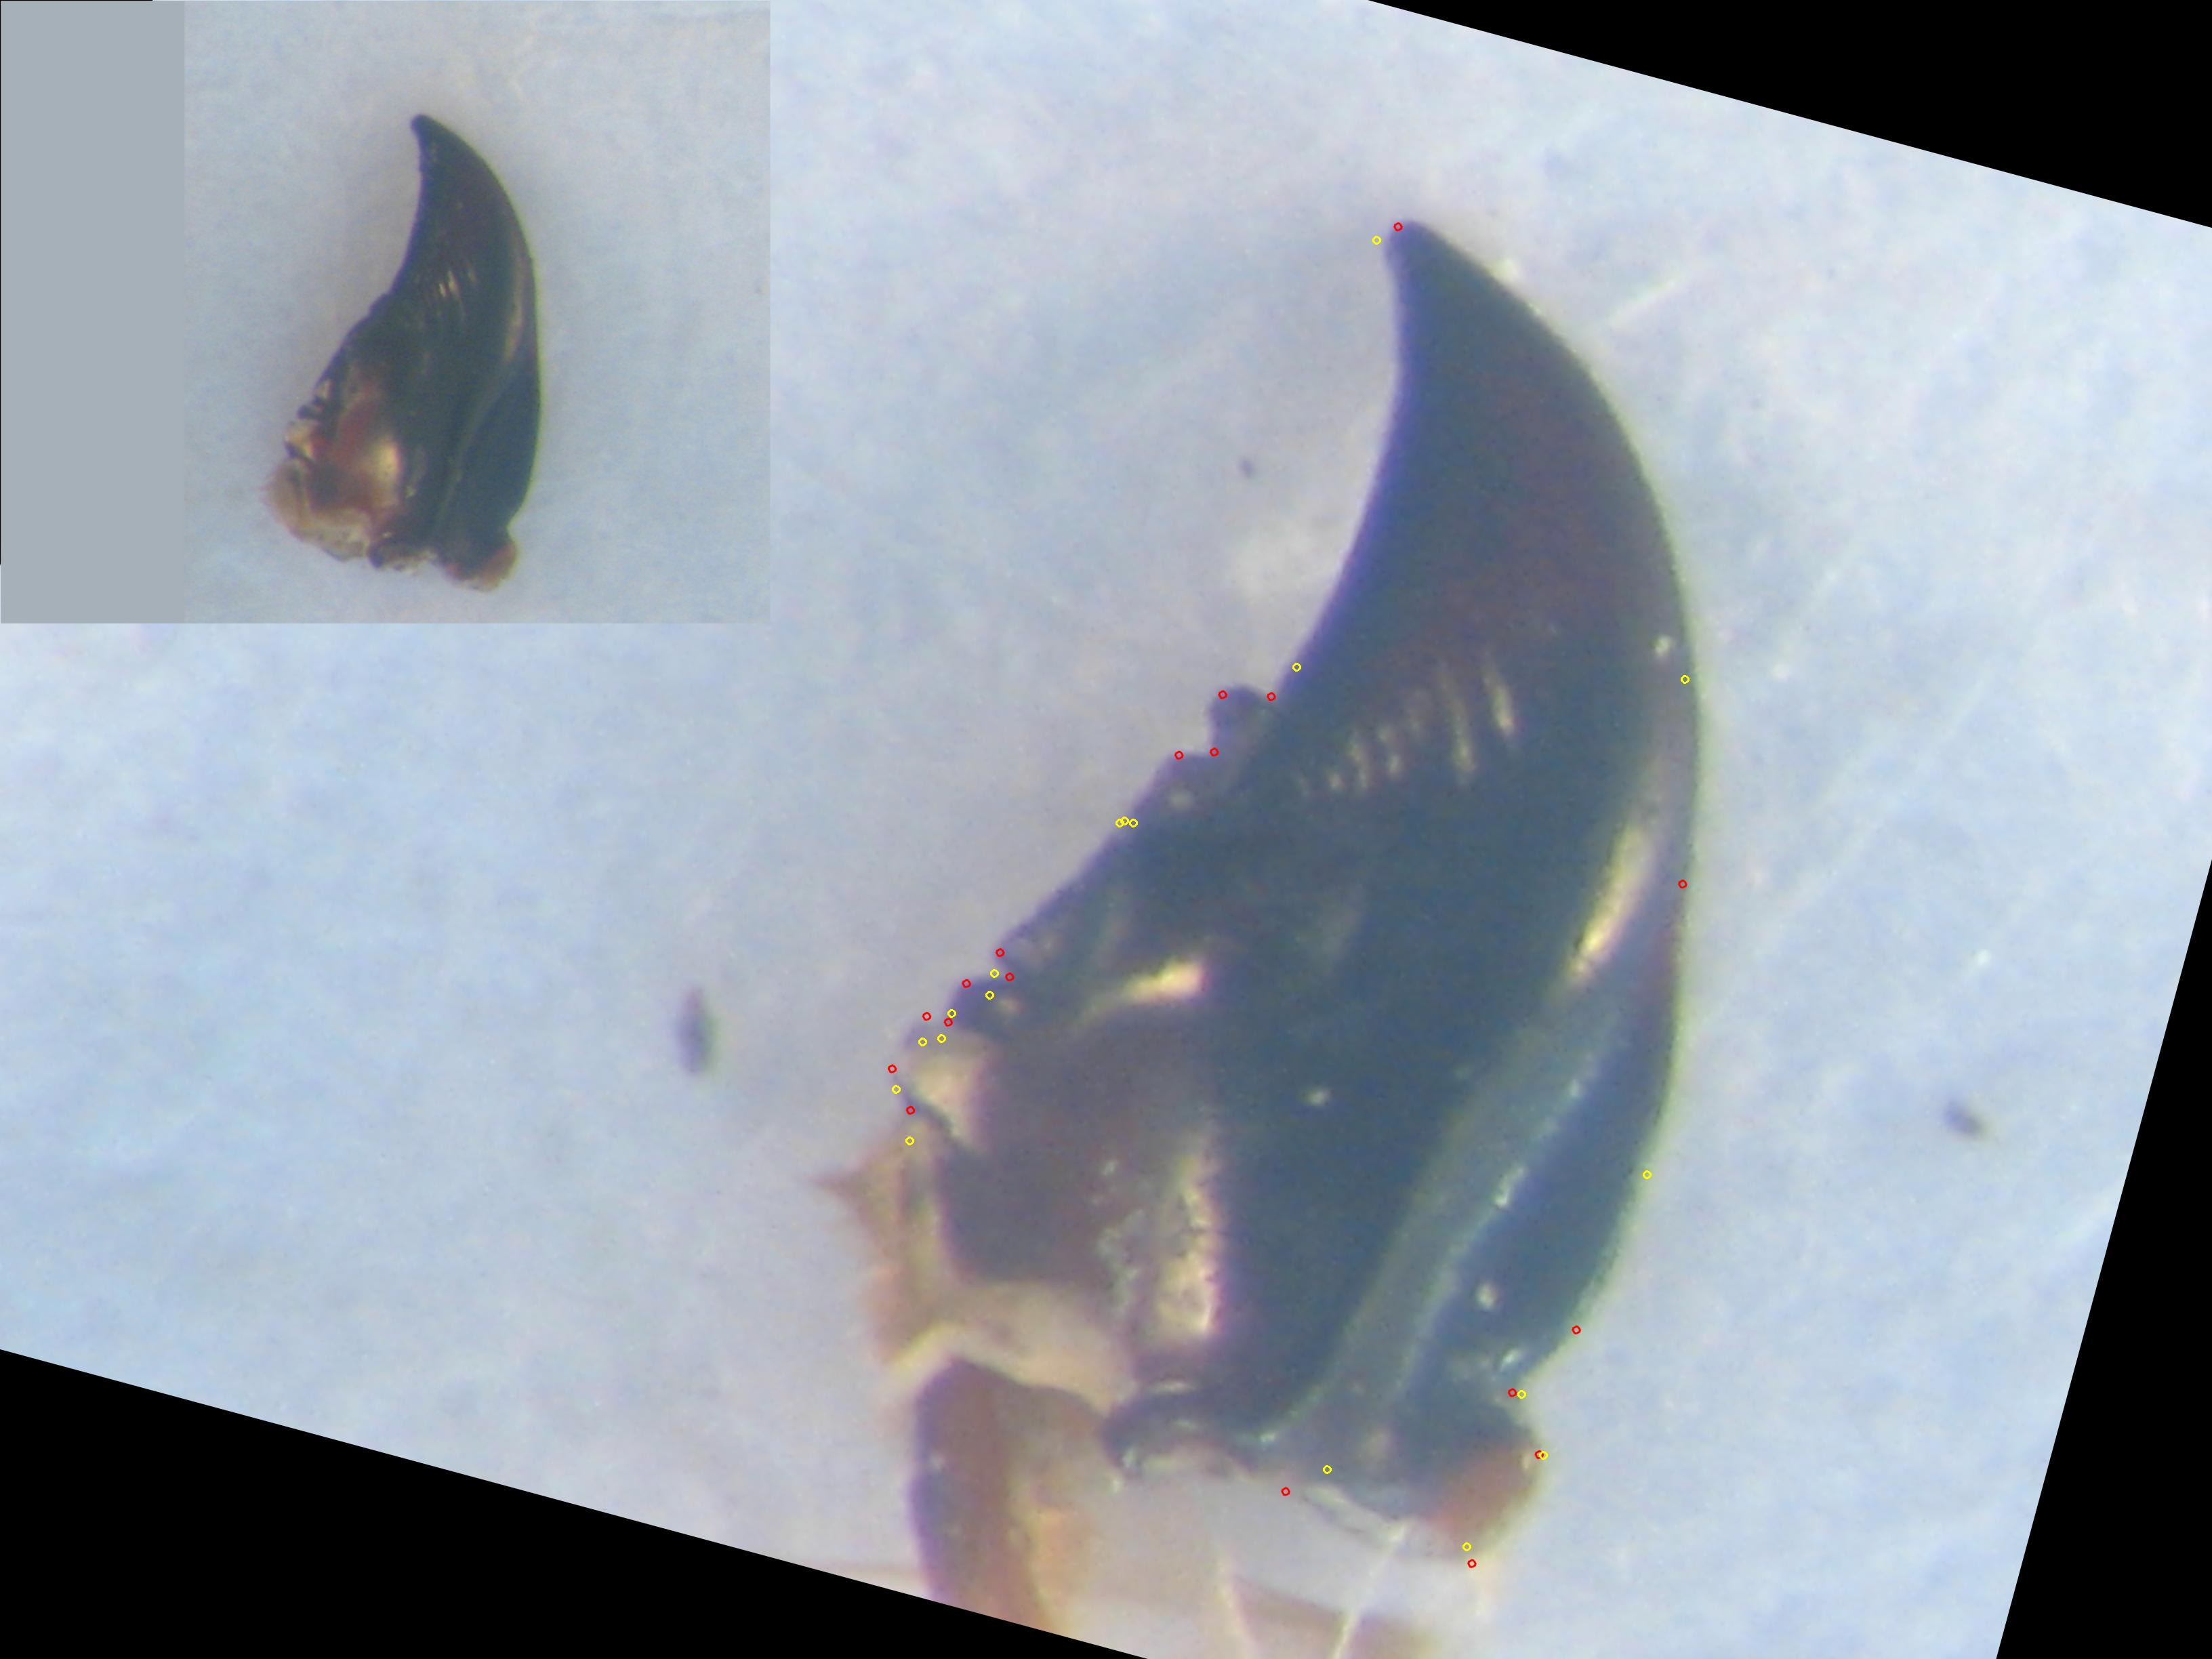
\includegraphics[height=8cm]{images/est19.JPG}	
	\end{center}
\end{frame}
\section{Result}
\begin{frame}{Result}
	\begin{itemize}
		\item Dataset: \textit{Mandibule droite} and \textit{mandibule gauche}
		\item Method includes 4 steps. The result of each step can effect to next step.
		\item This method can be used to identify the landmarks. But, in some cases, the estimated landmarks are not close with manual landmarks.
	\end{itemize}
\end{frame}
\section{References}
\begin{frame}[allowframebreaks]{References}
	\begin{thebibliography}{10}
		\setbeamertemplate{bibliography item}[article]
		\bibitem{palaniswamy}
		Palaniswamy, Sasirekha, Neil A. Thacker, and Christian Peter Klingenberg
		\newblock Automatic identification of landmarks in digital images
		\newblock {\em IET Computer Vision}, 4.4 (2010): 247-260
		
		\setbeamertemplate{bibliography item}[article]		
		\bibitem{pgh}
		Thacker, Neil A., P. A. Riocreux, and R. B. Yates. 
		\newblock "Assessing the completeness properties of pairwise geometric histograms." 
		\newblock{\em Image and Vision Computing}, 13.5 (1995): 423-429.
	\end{thebibliography}
\end{frame}
\begin{frame}[plain]
  \Huge{\centerline{Thank you !}}
\end{frame}
\end{document}